\documentclass[xcolor={table}, fleqn]{beamer}
%\usetheme{singapore}
\usepackage{bm}
\usepackage{listings,verbatim}
\usepackage{fancyvrb,tikz,color,xcolor,colortbl}
\usepackage{hyperref,booktabs,tabularx,float}
\usepackage{multirow,soul}
\newcommand{\hlc}[2][yellow]{{\sethlcolor{#1} \hl{#2}}}
%\usepackage[table]{xcolor}
%\usepackage{verbatim}
% \usepackage{array}
%\lstloadlanguages{R}
%\lstset{ language=R, basicstyle=\scriptsize\ttfamily, commentstyle=\ttfamily\color{gray}, numbers=left, numberstyle=\ttfamily\color{gray}\footnotesize, stepnumber=1, numbersep=5pt, backgroundcolor=\color{white}, showspaces=false, showstringspaces=false, showtabs=false, frame=single, tabsize=2, captionpos=b, breaklines=true, breakatwhitespace=false, escapeinside={}, keywordstyle={}, morekeywords={} }\renewcommand{\P}{\mathcal{P}}
%\newcommand{\bt}{\pmb{\theta}}
%\newcommand{\bG}{\pmb{\Gamma}}
\newcommand{\p}{\pause}
\definecolor{Grey}{rgb}{0.95,0.95,0.95}
\definecolor{male}{rgb}{1,.8,1}
\definecolor{female}{rgb}{.8,1,.8}
\newcommand{\male}[1]{\colorbox{male}{#1}}
\newcommand{\female}[1]{\colorbox{female}{#1}}
\newcommand{\pitem}{\pause \item}
\newenvironment{graytext}{\color{gray}}{\ignorespacesafterend}

\newcommand\independent{\protect\mathpalette{\protect\independenT}{\perp}}
\def\independenT#1#2{\mathrel{\rlap{$#1#2$}\mkern2mu{#1#2}}}

\definecolor{umassblue}{RGB}{51,51,153}
\definecolor{umassgreen}{RGB}{0,102,102}
%\definecolor{blue}{RGB}{51,51,153}
\definecolor{bblue}{RGB}{0,0,255}
\definecolor{red}{RGB}{153,0,51}

\newcommand\verbbf[1]{\textcolor[RGB]{51,51,153}{\textbf{$\blacksquare$ #1}}}
\newcommand\verbrf[1]{\textcolor[RGB]{153,0,51}{\textbf{$\blacksquare$ #1}}}

\newcommand{\N}{\mathcal{N}}
\newcommand{\Y}{\bm{\mathcal{Y}}} 

\usefonttheme{serif}

\newenvironment{changemargin}[2]{%
  \begin{list}{}{%
    \setlength{\topsep}{0pt}%
    \setlength{\leftmargin}{#1}%
    \setlength{\rightmargin}{#2}%
    \setlength{\listparindent}{\parindent}%
    \setlength{\itemindent}{\parindent}%
    \setlength{\parsep}{\parskip}%
  }%
  \item[]}{\end{list}} 

%
\title{\LARGE Reading between the Emails: Gendered Patterns of Communication in Local Government}
%
\definecolor{umassred}{HTML}{8C2633}
\setbeamercolor{structure}{fg=umassblue} 
\author{\large\textbf{Matthew J. Denny}}

%\affil[1]{University of Massachusetts Amherst}
%\affil[2]{University of Connecticut}

\institute{\large Penn State University --- 
 \texttt{mdenny@psu.edu}\\
 \color{blue}\texttt{www.mjdenny.com}\\ 
 \texttt{@MatthewJDenny}
}

\date{Collaborators: James ben Aaron, Hanna Wallach,\\ Bruce A. Desmarais\\~\\
\begin{tabular}{cc}
\hspace*{-.2in} \tiny \begin{minipage}{3in}
\large  Supported by NSF Grants: DGE-1144860, and CISE-1320219\\~\\
\end{minipage}
& \includegraphics[scale=.05]{./images/NSF_logo.png}
\end{tabular}
}
\begin{document}

%{
%\usebackgroundtemplate{
\includegraphics[width=\paperwidth]{./images/cat.jpg}}%
\begin{frame}
  \titlepage
\end{frame}
%}

% \begin{frame}\frametitle{Gender and Communication in Local Government}
% 	\LARGE
% 	\begin{itemize}
% 		\item Gender bias in organizations.
% 		\vspace*{.3in}
% 		\item How does gender shape communication?
% 		\vspace*{.3in}
% 		\item Differences across domains?
% 		\vspace*{.3in}
% 		\item Relation to previous findings?
% 	\end{itemize}
% \end{frame}

\begin{frame}\frametitle{Research Question}
	\LARGE
	How does the relationship between gender and the pattern of communication vary across organizational domains? 
\end{frame}


% \begin{frame}\frametitle{Challenges and Opportunities}
% 	\LARGE
% 	\begin{itemize}
% 		\item Observational and self report data.
% 		\vspace*{.15in}
% 		\begin{itemize}
% 			\LARGE
% 			\item Restricted in scope. Biased?
% 		\end{itemize}
% 		\vspace*{.15in}
% 		\item Electronic communication data.
% 		\vspace*{.15in}
% 		\begin{itemize}
% 			\LARGE
% 			\item Primary source, day-to-day.
% 			\vspace*{.15in}
% 			\item Public records laws.
% 		\end{itemize}
% 		\vspace*{.15in}
% 		\item Study micro-level interactions.
% 	\end{itemize}
%
% \end{frame}

\begin{frame}\frametitle{Previous Research}
	\LARGE
% No previous research on gender in organizations has had access to micro level behavioral data, it has relied on administrative data or self reports.
	% \begin{changemargin}{-1cm}{ -1cm}
%     \centering
% 	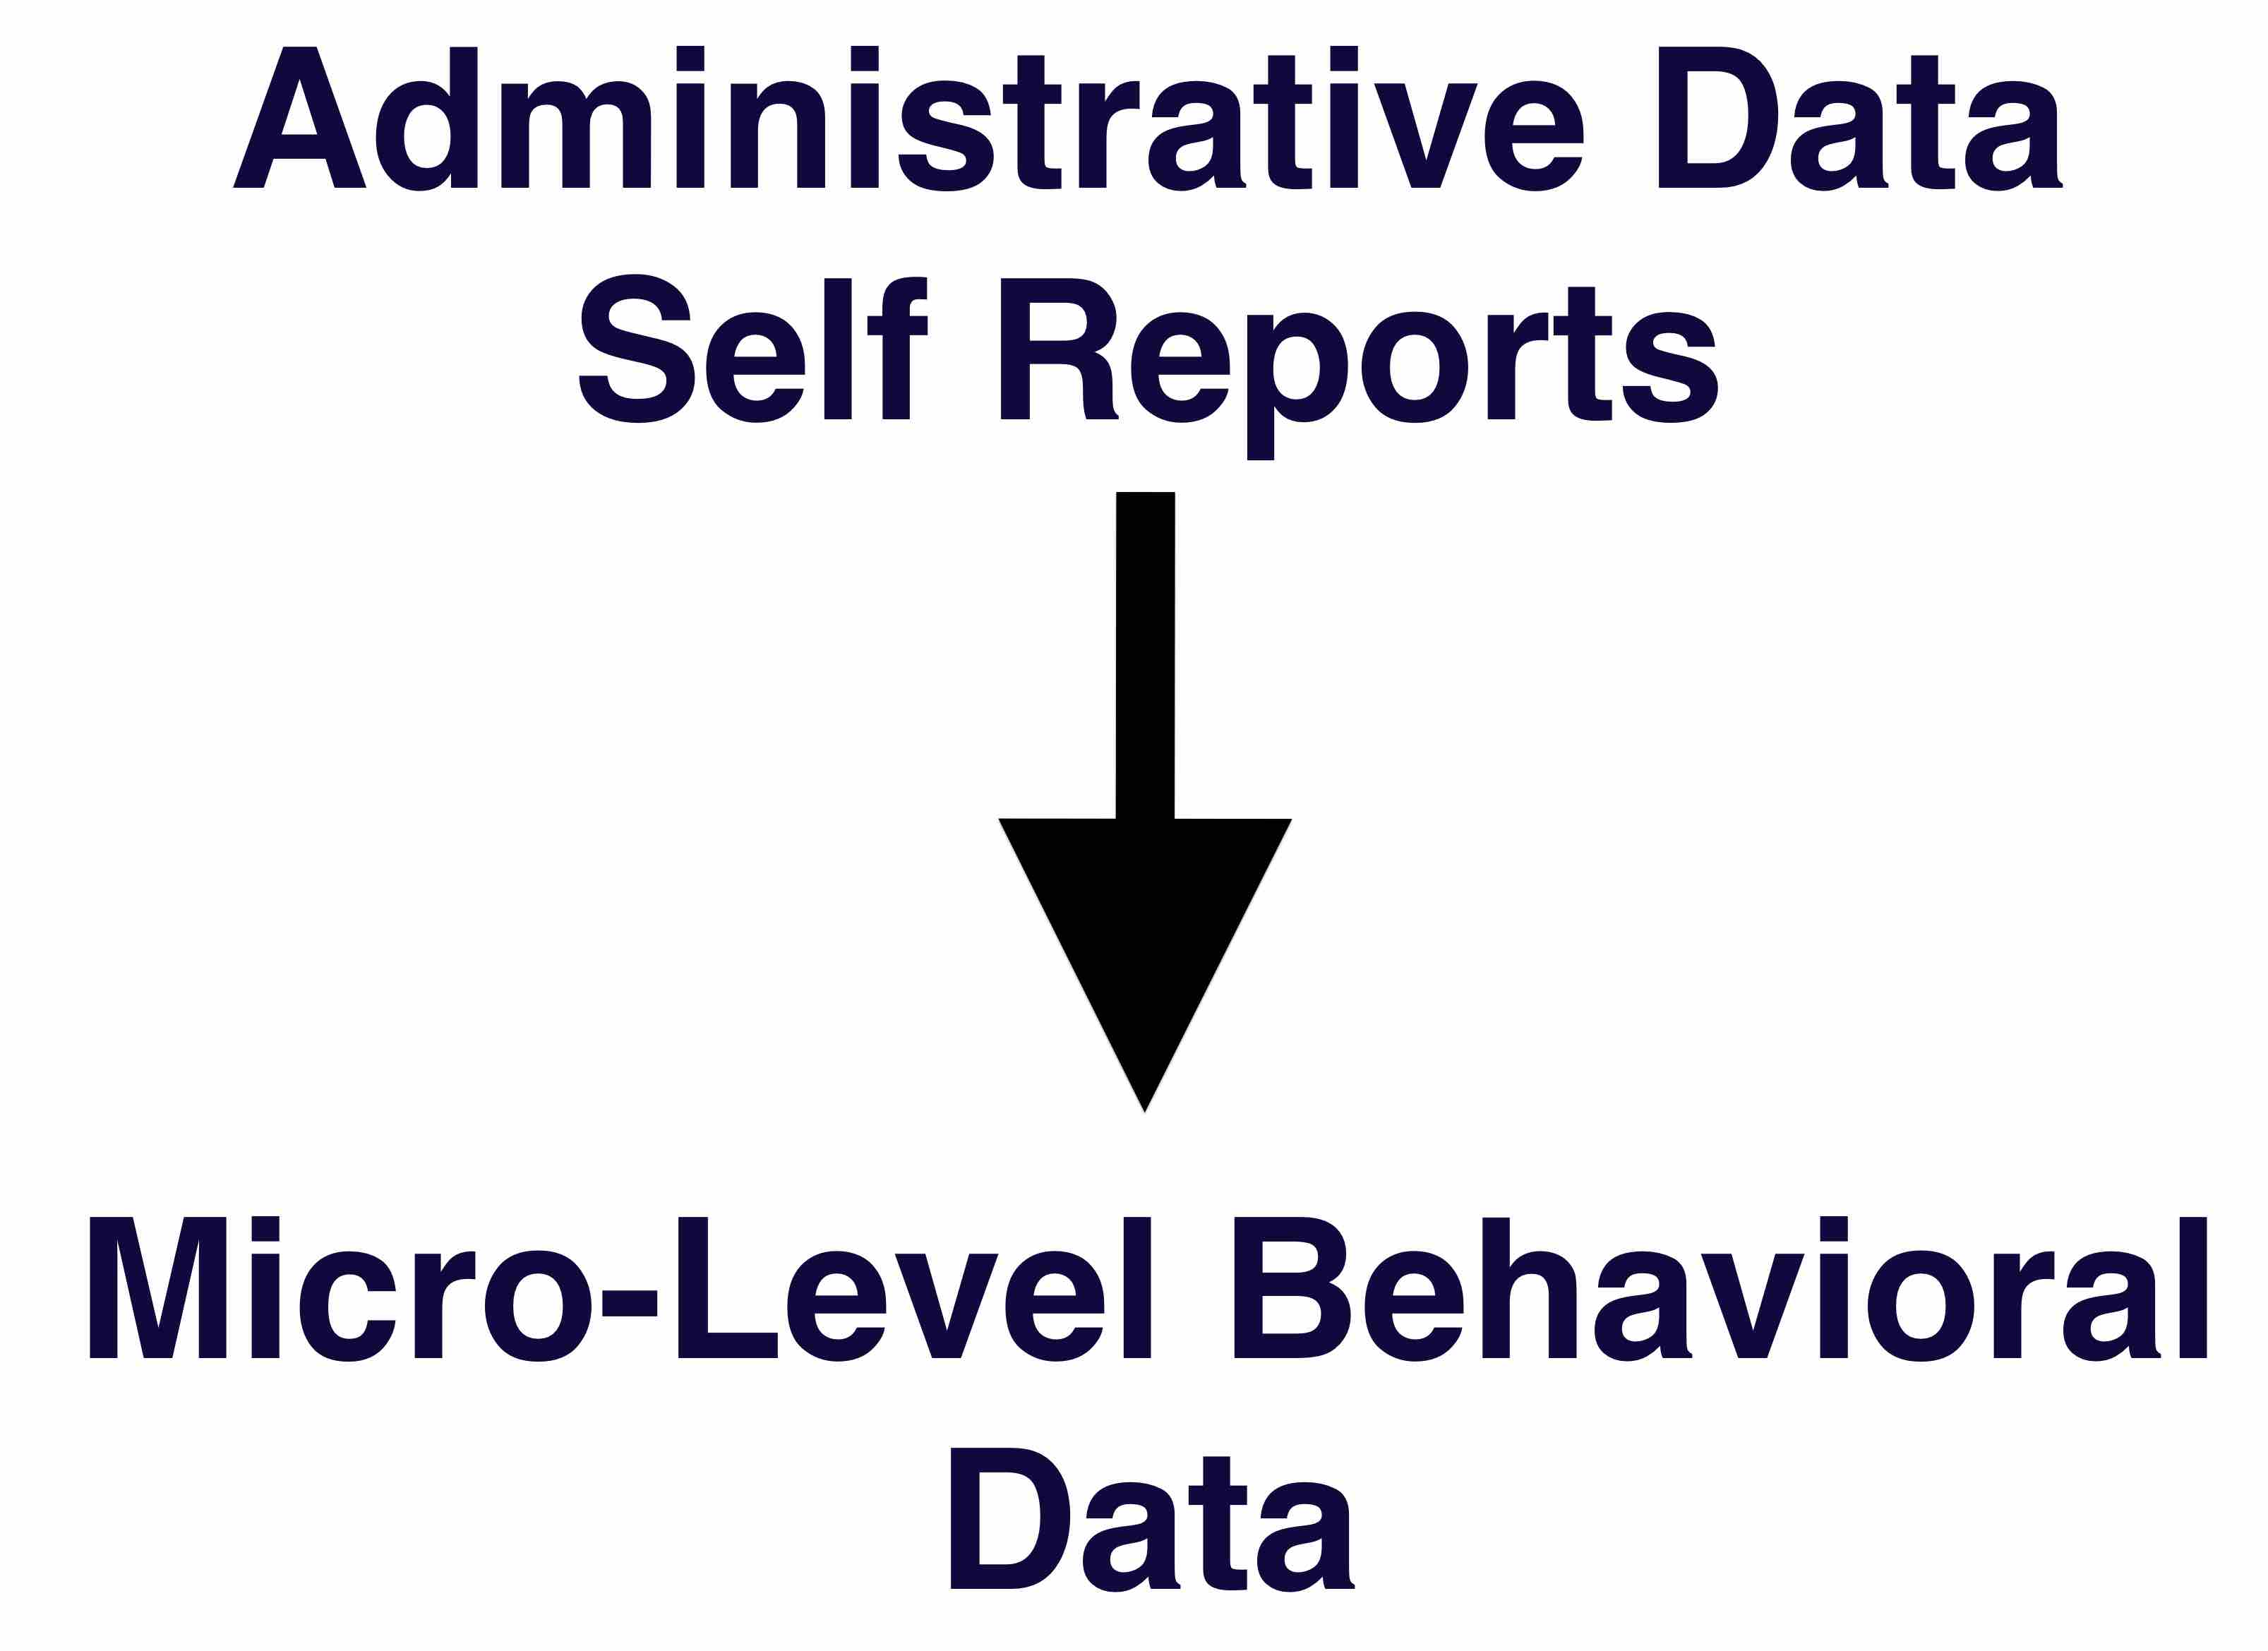
\includegraphics[width=0.98\textwidth]{images/New_Data.jpg}
% 	\end{changemargin}
\begin{itemize}
	\item Administrative Data
	\vspace*{.2in}
	\begin{itemize}
		\LARGE
		\item Salary, position, education, etc.
	\end{itemize}
	\vspace*{.2in}
	\item Self Reports
	\vspace*{.2in}
	\begin{itemize}
		\LARGE
		\item Surveys
		\vspace*{.2in}
		\item Interviews
	\end{itemize}
\end{itemize}

\end{frame}

\begin{frame}\frametitle{}
	\begin{center}
		\Huge\textbf{Public Domain Email Data}
	\end{center}
\end{frame}

\begin{frame}\frametitle{County Government Email Data}
	\Large
	\begin{itemize}
		\item Public records requests.
		\vspace*{.1in}
		\item Department manager email data from 17 North Carolina Counties.
		\vspace*{.1in}
		\item 500,000 emails, 17,000 between managers.
		\vspace*{.1in}
	\end{itemize}
	\centering
	
\includegraphics[width=0.95\textwidth]{images/County_Map.pdf}
\end{frame}


\begin{frame}[plain]
	\Large
\begin{changemargin}{-1cm}{ -1cm}		  
	  \centering
	  \begin{tabular}{lrrrr}
	    \toprule
	    & \multicolumn{2}{c}{Manager Gender} & \\
	    \cmidrule{2-3}
	    County & Male & Female & \# Emails  \\
	    \midrule
	    Alexander & 12 & 9 & 907   \\
	    Caldwell & 12 & 8 & 121     \\
	    Chowan & 12 & 11 & 2,027   \\
	    Columbus & 14 & 10 & 920   \\
	    Dare & 15 & 12 & 2,247    \\
	    %Duplin & 13 & 14 & 1,914    \\
	    % Hoke & 13 & 11 & 1,106  \\
  % 	    Jackson & 18 & 6 & 1,499    \\
		\vdots & \vdots & \vdots & \vdots \\
	    % Lenoir & 15 & 5 & 560  \\
% 	    Lincoln & 15 & 7 & 573   \\
% 	    McDowell & 12 & 5 & 326   \\
% 	    Montgomery & 8 & 10 & 680   \\
% 	    Nash & 11 & 8 & 1,147  \\
	    % Person & 12 & 9 & 1,491   \\
	    Transylvania & 16 & 4 & 1,857  \\
	    Vance & 10 & 8 & 185   \\
	    Wilkes & 15 & 2 & 303   \\
	    \midrule
	    Total & 223 & 139 & 17,863 \\
	    \bottomrule
	  \end{tabular}

\end{changemargin}

\end{frame}

% \begin{frame}\frametitle{}
% 	\begin{center}
% 		\Huge\textbf{Aggregate Analysis}
% 	\end{center}
% \end{frame}
%
% \begin{frame}\frametitle{Aggregate Patterns}
%
% 	\begin{changemargin}{-1cm}{ -1cm}
% 	\Large
% 	\centering
%     \begin{tabular}{lrrr}
%       \toprule
%       & \multicolumn{2}{c}{Manager Gender} \\
%       \cmidrule{2-3}
%       & Male & Female  \\
%       \midrule
%       Average \# emails sent & 48.3 & 51 \\
%       Average \# recipients per email sent & 1.45 & 1.43 \\
%       \midrule
%       Average \# emails received & 70.8 & 71.6 \\
%       \bottomrule
%     \end{tabular}
% 	\end{changemargin}
%
% 	\bigskip
% 	\centering
% 	\Large
%
%
% 	\LARGE
% 	\begin{itemize}
% 		\item Mild gender-heterophily.
% 	\end{itemize}
%
% 	% \begin{tabular}{rlrrr}
% % 	  \toprule
% % 		 && \multicolumn{2}{c}{Recipient} \\
% % 		\cmidrule{3-4}
% % 	& & Male & Female & Total  \\
% % 		 \midrule
% % 		\multirow{2}{*}{Sender} & Male & 7,299 & 6,286 & 13,585 \\
% % 	& Female & 5,325 & 3,510 & 8,835 \\
% % 	\midrule
% % 		 & Total & 12,624 & 9,796 & \\
% % 		\bottomrule
% % 		\end{tabular}
%
% \end{frame}




\begin{frame}\frametitle{}
	\begin{center}
		\Huge\textbf{Department Affiliation as Domain}
	\end{center}
\end{frame}

\begin{frame}\frametitle{Individual Department Gender Breakdown}
	
	\begin{changemargin}{-1cm}{ -1cm}
		\Large
    \centering
	\setlength{\tabcolsep}{3pt}
	  \begin{tabular}{rrrrrrrrrrrrrrrrrrrrrrrr}
	    \toprule
	
		   & \cellcolor{male} \rotatebox{90}{Emergency} & \cellcolor{male}\rotatebox{90}{Manager} & \cellcolor{female}\rotatebox{90}{HR} & \cellcolor{female}\rotatebox{90}{Finance} & \cellcolor{male}\rotatebox{90}{IT} & \rotatebox{90}{Health} & \cellcolor{male}\rotatebox{90}{Plan/Dev} & \cellcolor{male}\rotatebox{90}{Util/Waste} & \rotatebox{90}{Tax} & \rotatebox{90}{Parks/Rec} & \rotatebox{90}{Soc\_Serv} & \cellcolor{male}\rotatebox{90}{Transport} & \cellcolor{female}\rotatebox{90}{Info} & \cellcolor{male}\rotatebox{90}{Misc} & \cellcolor{male}\rotatebox{90}{Inspections} \\ % & \rotatebox{90}{Maintenance} & \rotatebox{90}{Library} & \rotatebox{90}{Veterans} & \rotatebox{90}{Seniors} & \rotatebox{90}{Animal}  \\ 
		     \midrule
		   Male & \cellcolor{male}29 & \cellcolor{male}15 & \cellcolor{female}3 & \cellcolor{female}5 & \cellcolor{male}11 & 6 & \cellcolor{male}17 & \cellcolor{male}15 & 11 & 9 & 8 & \cellcolor{male}8 & \cellcolor{female}2 & \cellcolor{male}5 & \cellcolor{male}13 \\  %& 5 & 3 & 5 & 2 & 9  \\ 
		     Female & \cellcolor{male}3 & \cellcolor{male}2 & \cellcolor{female}12 & \cellcolor{female}12 & \cellcolor{male}2 & 11 & \cellcolor{male}6 & \cellcolor{male}2 & 7 & 5 & 10 & \cellcolor{male}1 & \cellcolor{female}6 & \cellcolor{male}2 & \cellcolor{male}3 \\% & 1 & 8 & 7 & 6 & 3  \\ 
			 \midrule
		     Total & \cellcolor{male}32 & \cellcolor{male}17 & \cellcolor{female}15 & \cellcolor{female}17 & \cellcolor{male}13 & 17 & \cellcolor{male}23 & \cellcolor{male}17 & 18 & 14 & 18 & \cellcolor{male}9 & \cellcolor{female}8 & \cellcolor{male}7 & \cellcolor{male}16 \\ %& 6 & 11 & 12 & 8 & 12 \\
	    \bottomrule
	    \end{tabular}
	\setlength{\tabcolsep}{6pt}
\bigskip
\bigskip

\begin{tabular}{ll}
	\cellcolor{male} Male dominated &
	\cellcolor{female} Female dominated
\end{tabular}


\end{changemargin} 
\end{frame}


\begin{frame}\frametitle{Does Gender Composition Matter?}
	\LARGE
Dasgupta et al. (2015). ``Female peers in small work groups enhance women’s motivation, verbal participation, and career aspirations in engineering". \emph{PNAS} \\~\\
\textbf{Are women more active in female dominated domains?}
\end{frame}

\begin{frame}\frametitle{Department-Dyad Regression Analysis}
	\LARGE
	\begin{itemize}
		\item Model department interaction.
		\vspace*{.3in}
		\item Base Model: Single Intercept
		\vspace*{.3in}
		\item Gender Model: Separate intercepts
		\vspace*{.15in}
		\begin{itemize}
			\LARGE
			\item MM, MF, FM, FF
		\end{itemize}
		\vspace*{.15in}
		\item Likelihood-Ratio Test.
	\end{itemize}
\end{frame}


\begin{frame}\frametitle{Female-Centric Dyads}
	\centering
	\Large
	\begin{tabular}{l}
	  \toprule
	FF $>$ FM $>$ MF $>$ MM  \\
	\hline
	  \female{HR} \& Health  \\ 
	  \female{HR} \& \male{Information Technology}  \\ 
	  \female{HR} \& \male{County Manager}  \\ 
	  \male{Planning} \& \female{HR} \\ 
	  Register of Deeds \& \female{HR}  \\ 
	  Parks and Recreation \& \female{HR}  \\ 
	  \female{Finance} \& \female{HR}  \\ 
	  \female{Finance} \& Parks and Recreation  \\ 
	  Social Services \& \female{HR}  \\ 
	  \male{Solid Waste and Recycling} \& \female{HR}  \\ 
	  Tax Administrator \& \female{HR}  \\ 
	   \bottomrule
	\end{tabular}
	
	
	
	
\end{frame}


\begin{frame}\frametitle{}
	\begin{center}
		\Huge\textbf{Email Content as Domain}
	\end{center}
\end{frame}


\begin{frame}\frametitle{A Generative Model for Email Data}
	\begin{changemargin}{-1cm}{ -1cm}
    \centering
	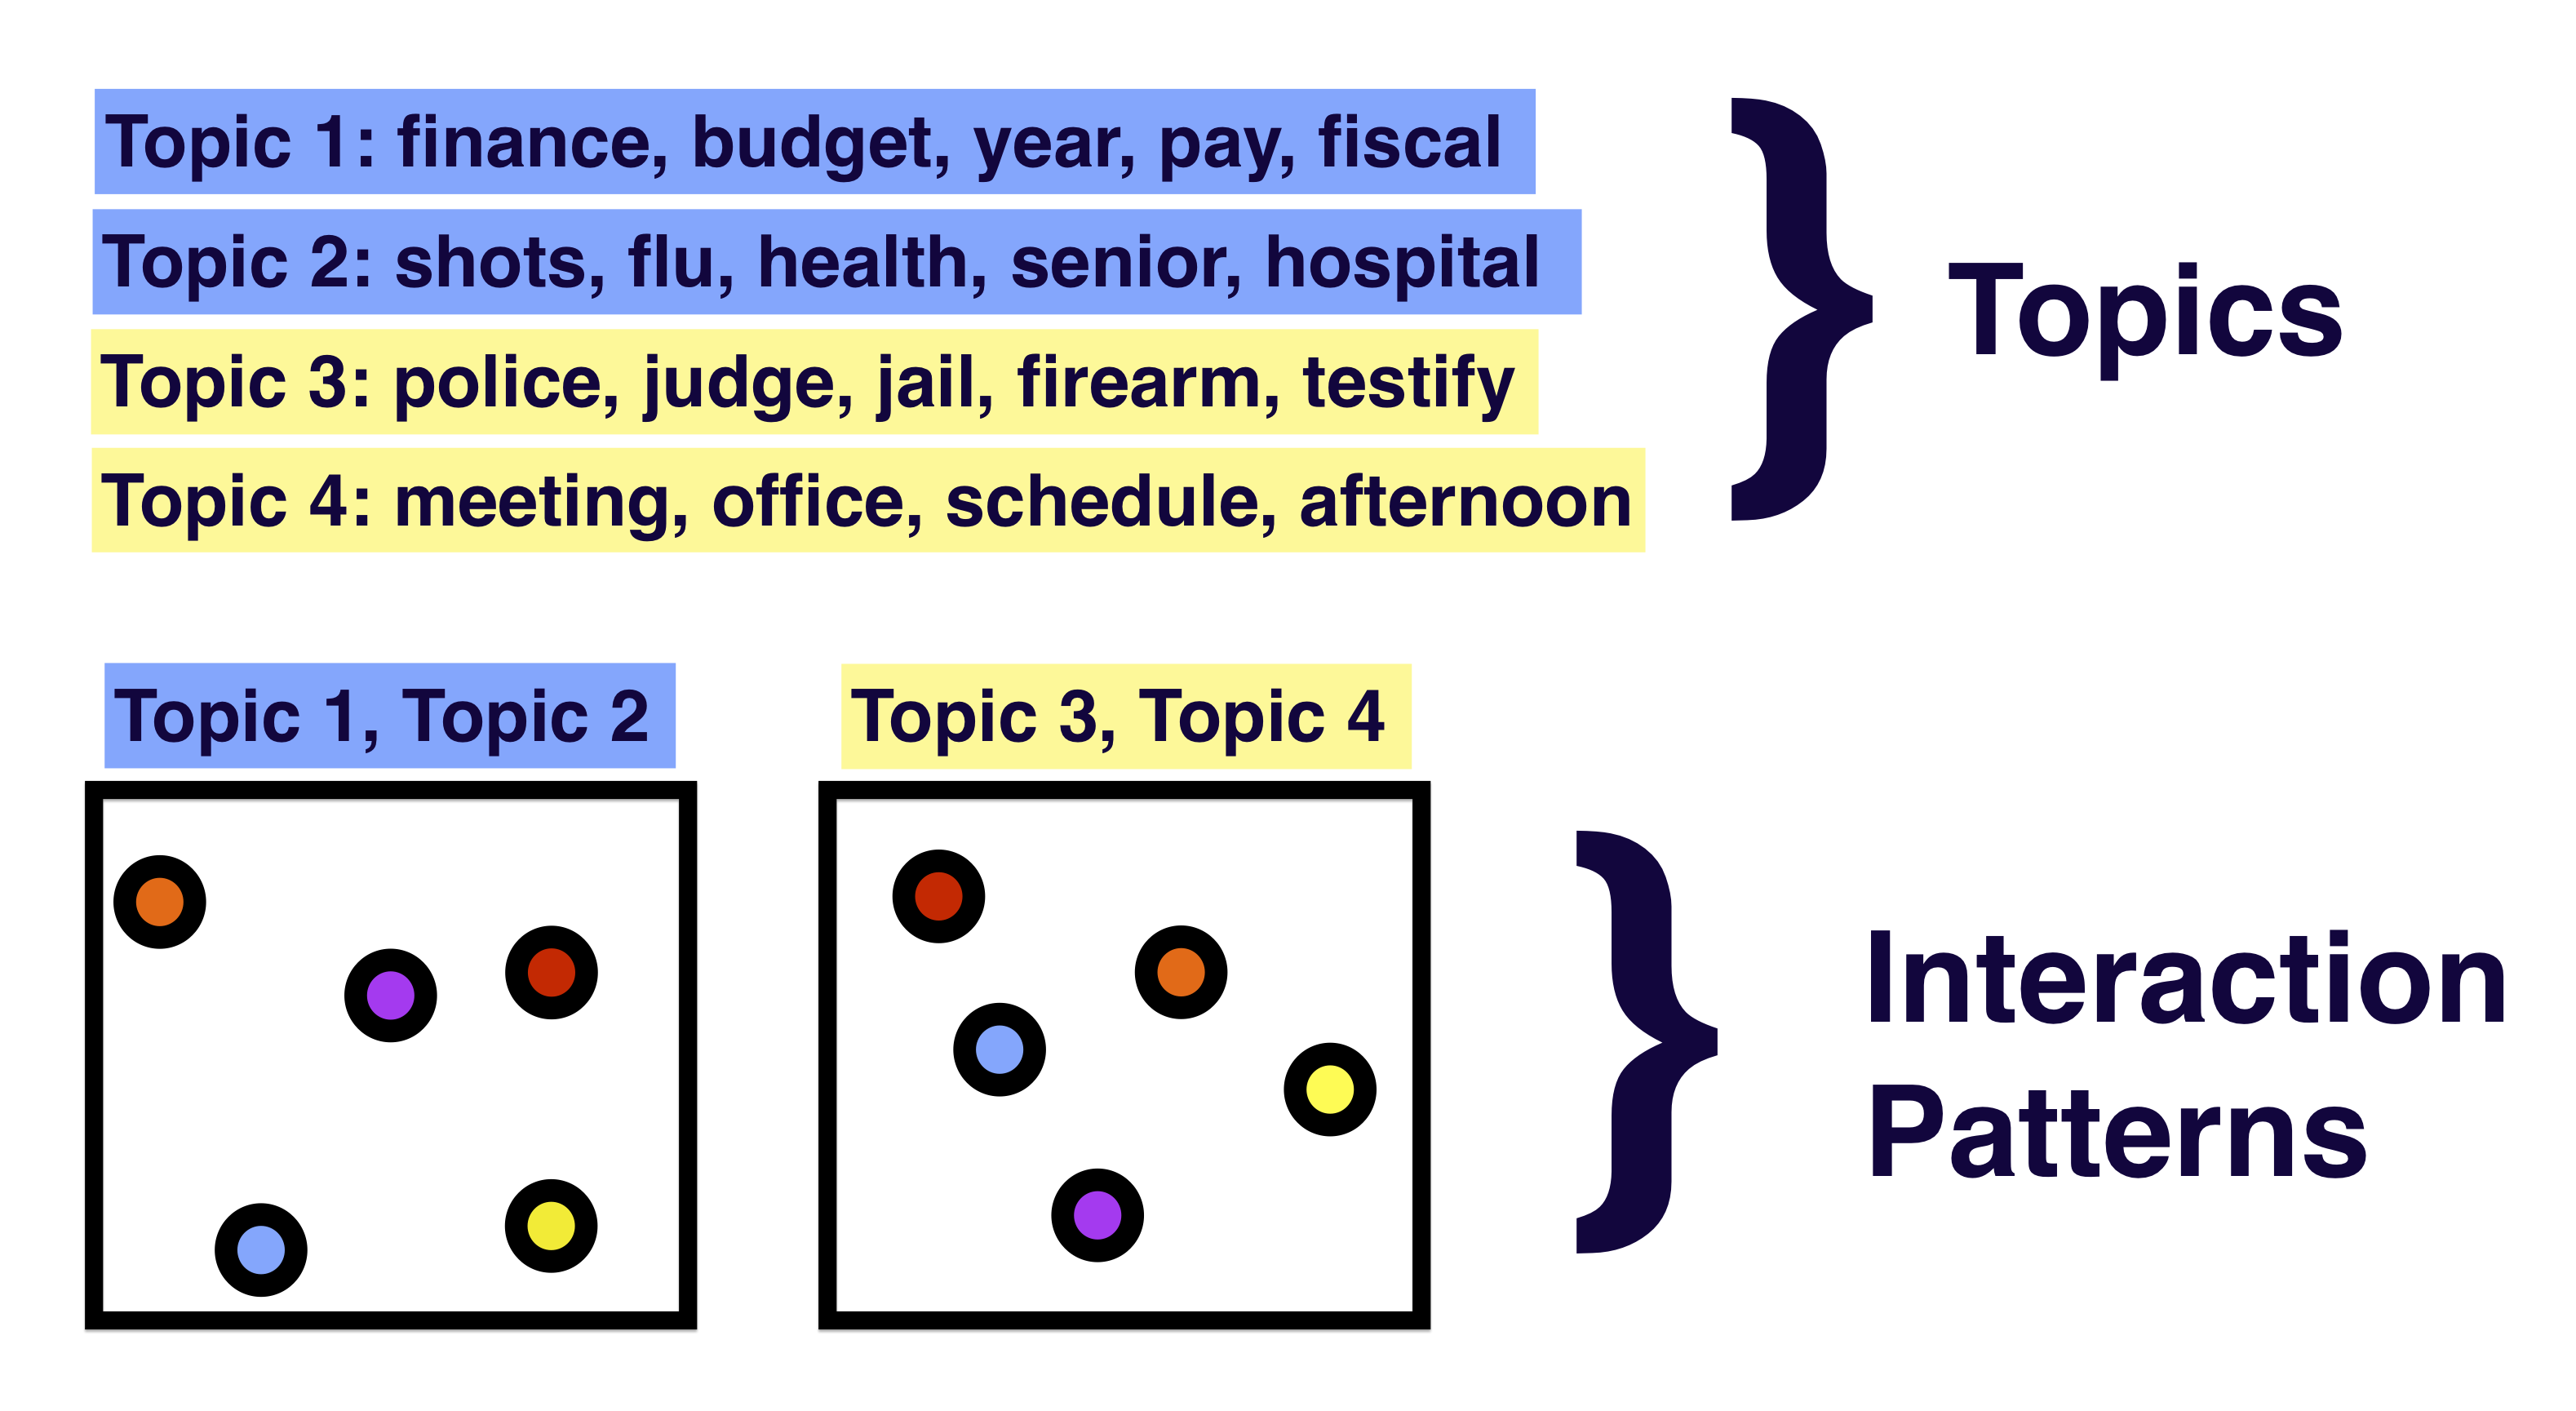
\includegraphics[width=1.15\textwidth]{images/Gen_Proc_1.png}
	\end{changemargin} 
\end{frame}


% \begin{frame}\frametitle{A Generative Model for Email Data}
% 	\begin{changemargin}{-1cm}{ -1cm}
%     \centering
% 	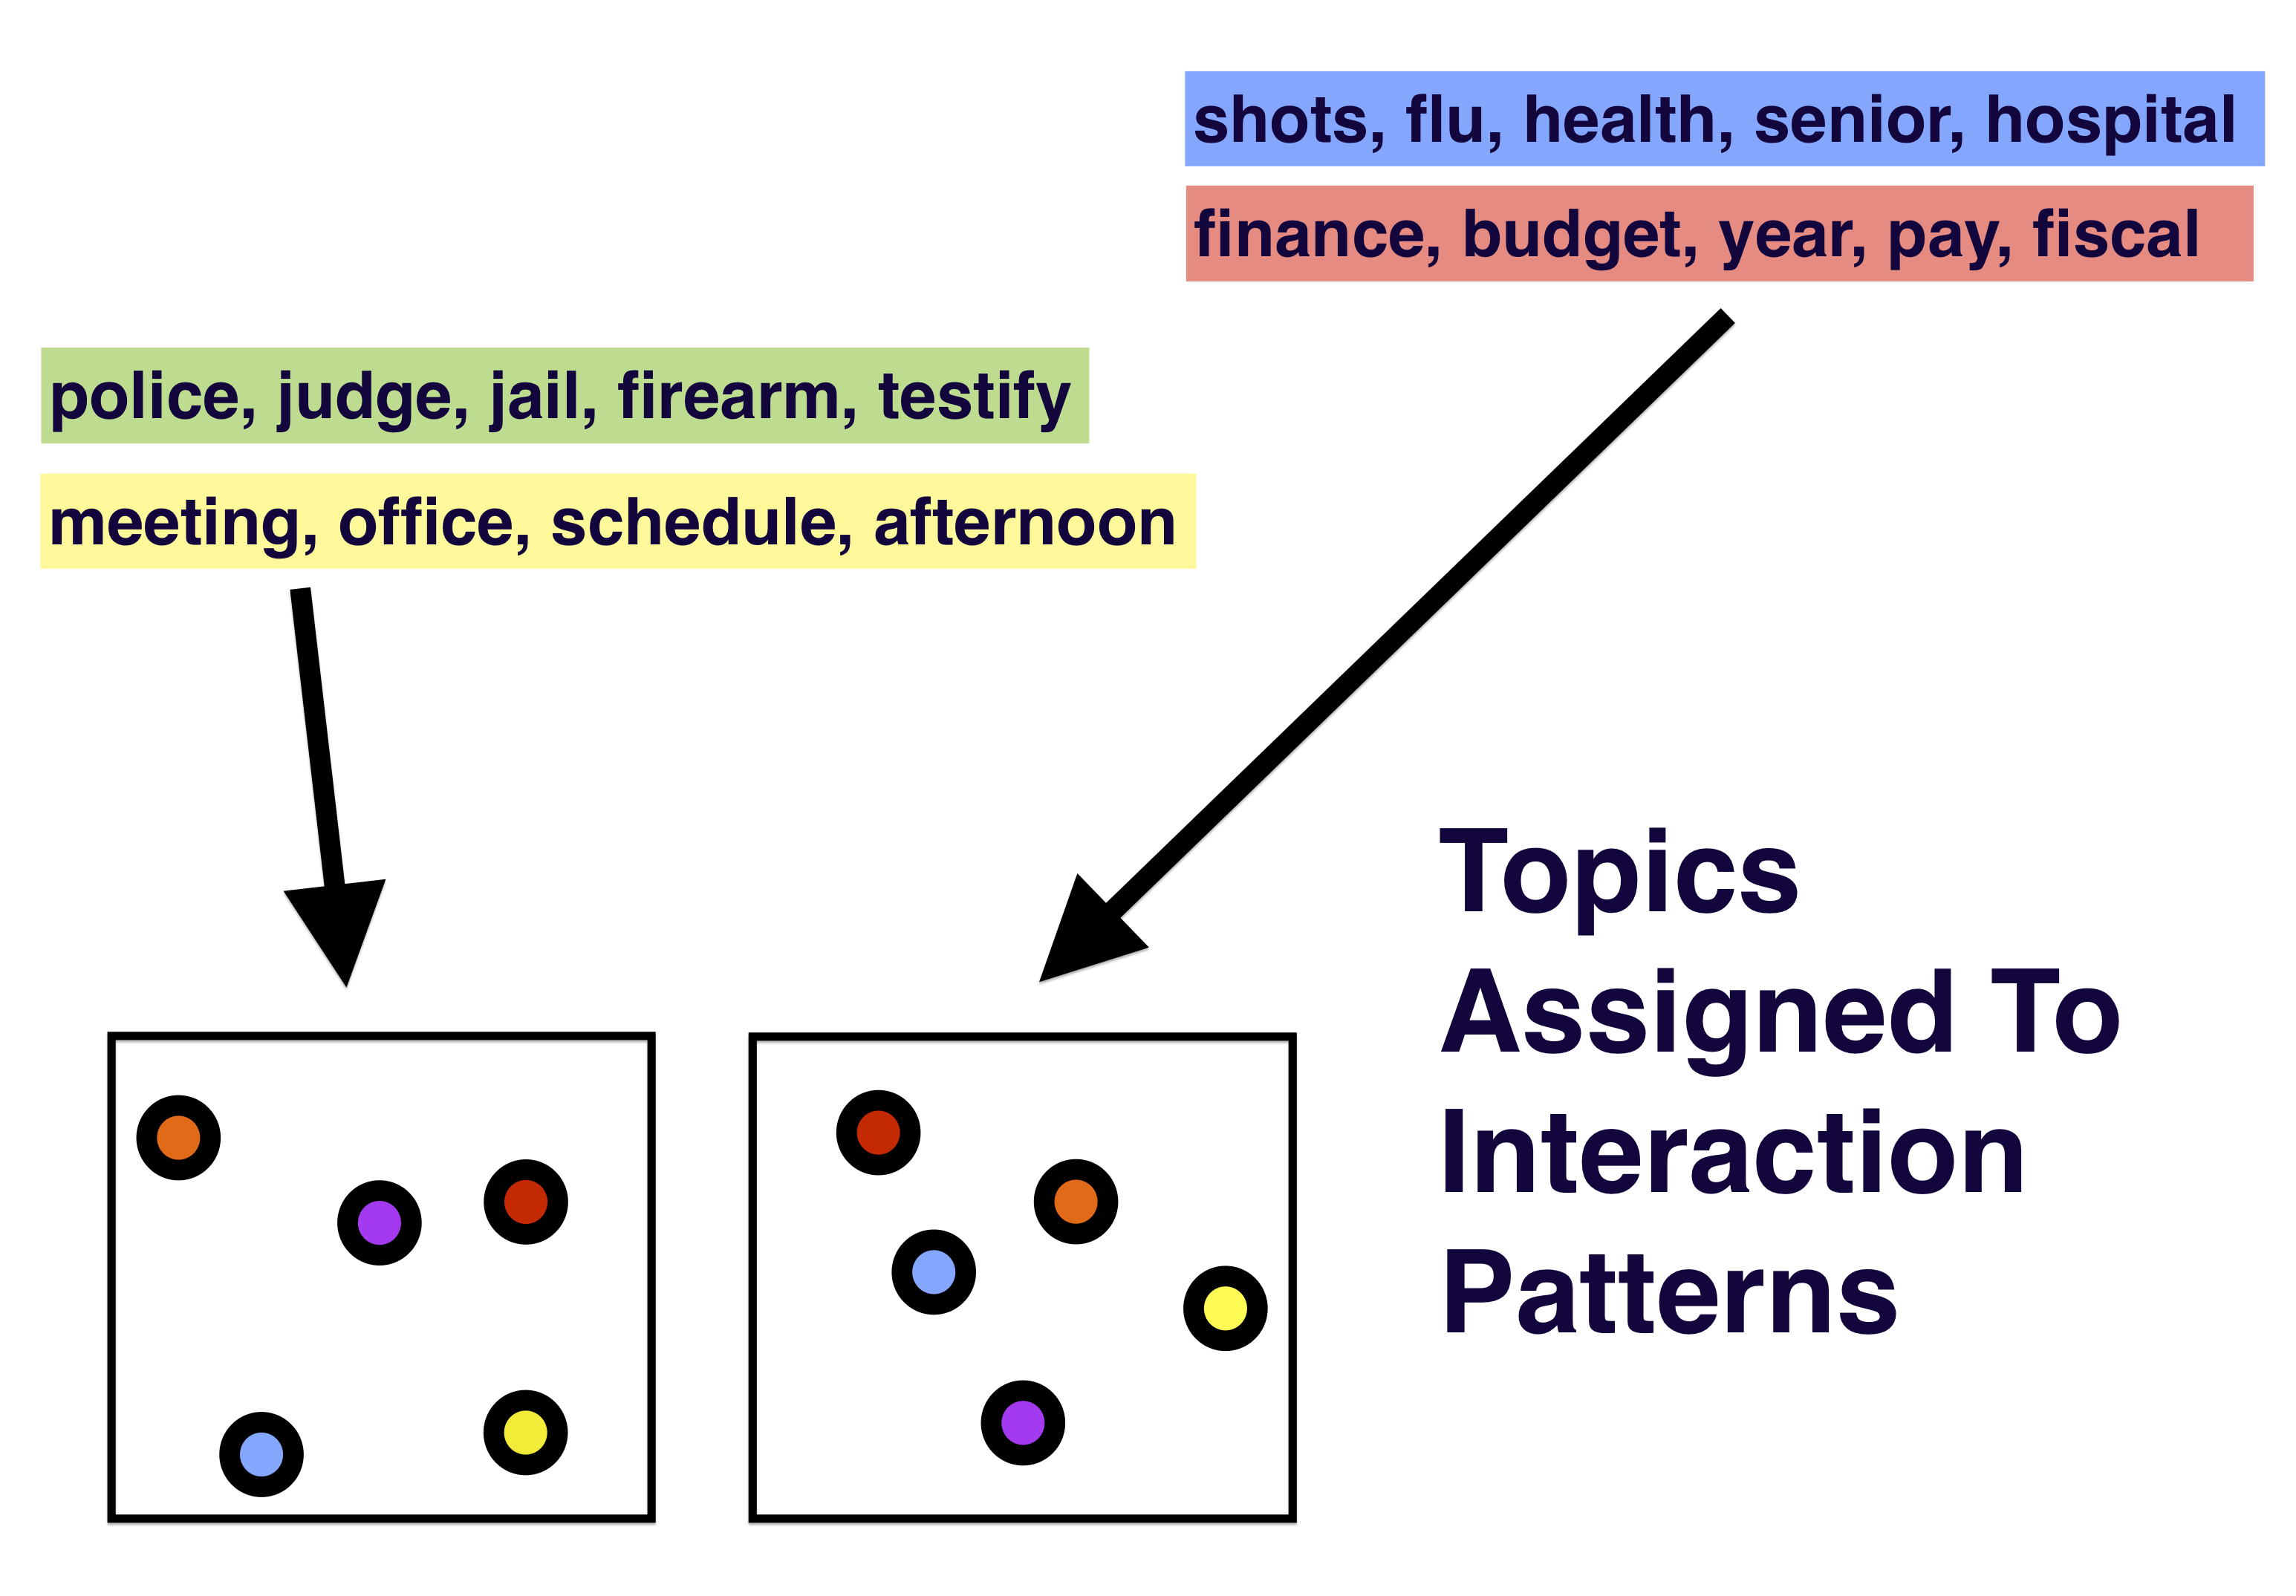
\includegraphics[width=0.98\textwidth]{images/Gen_Proc_1a.png}
% 	\end{changemargin}
% \end{frame}
%
% \begin{frame}\frametitle{A Generative Model for Email Data}
% 	\begin{changemargin}{-1cm}{ -1cm}
%     \centering
% 	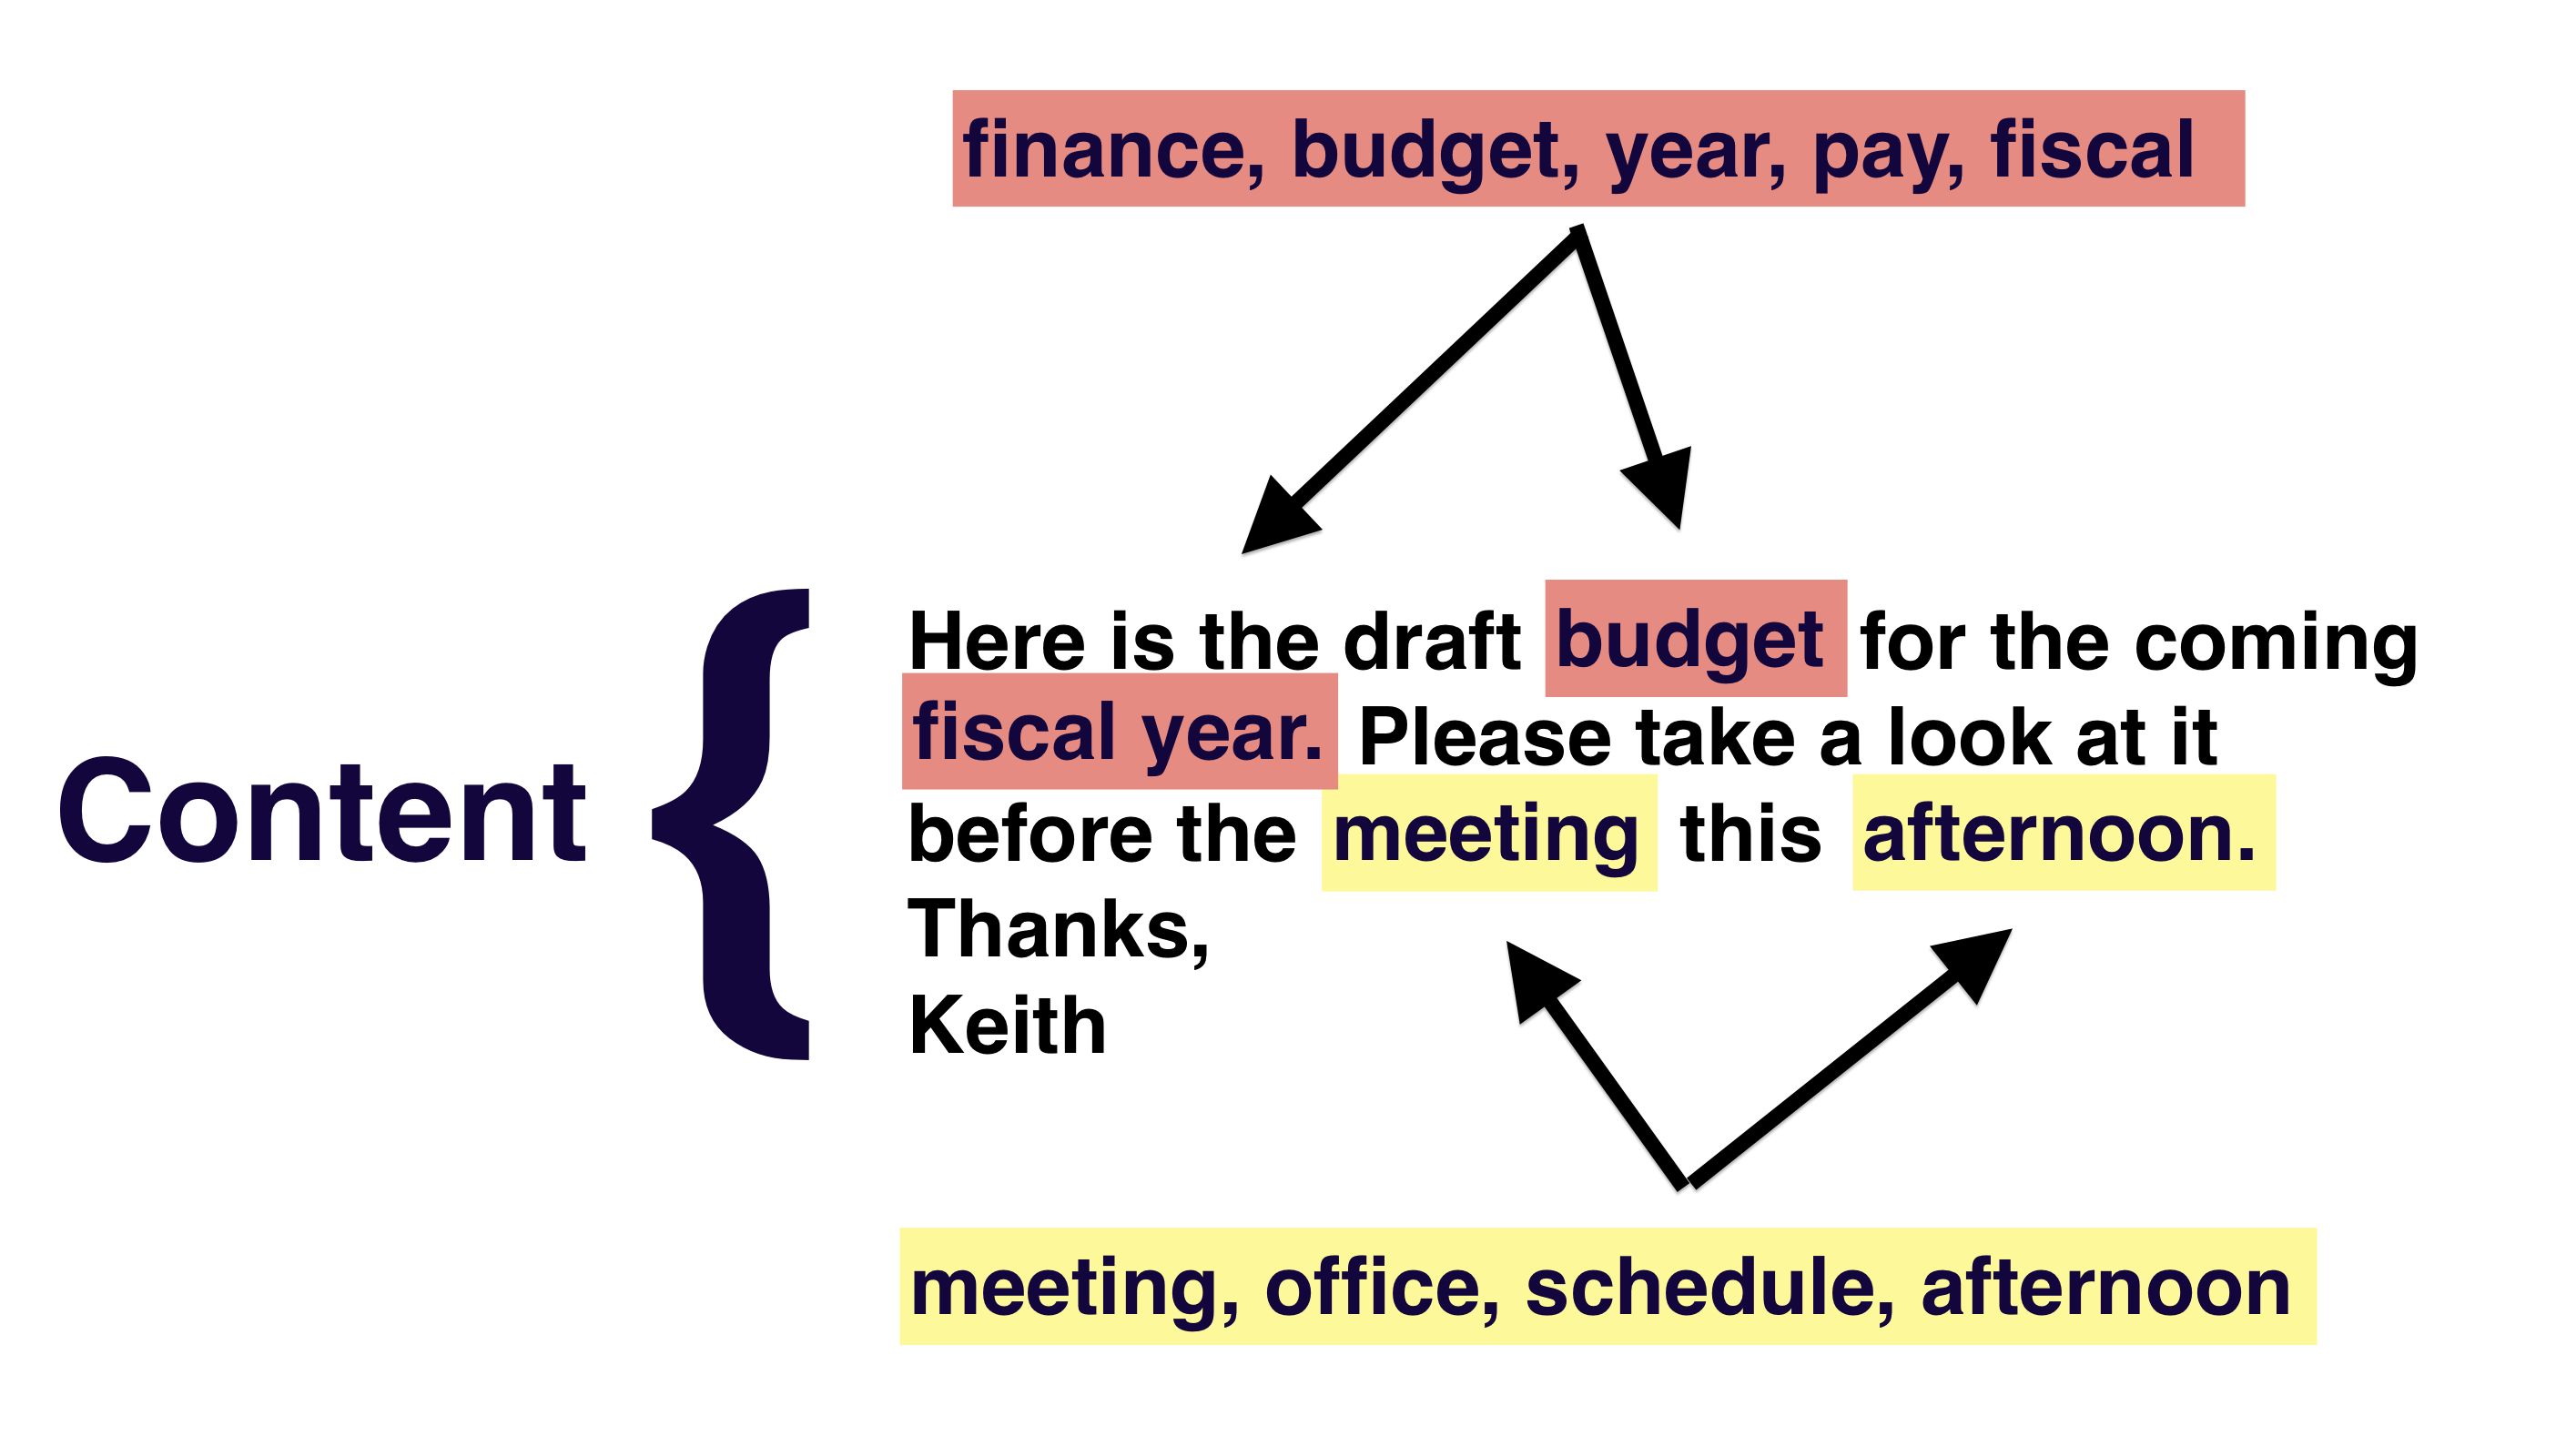
\includegraphics[width=0.98\textwidth]{images/Gen_Proc_2.png}
% 	\end{changemargin}
% \end{frame}


\begin{frame}\frametitle{A Generative Model for Email Data}
	\begin{changemargin}{-1cm}{ -1cm}
    \centering
	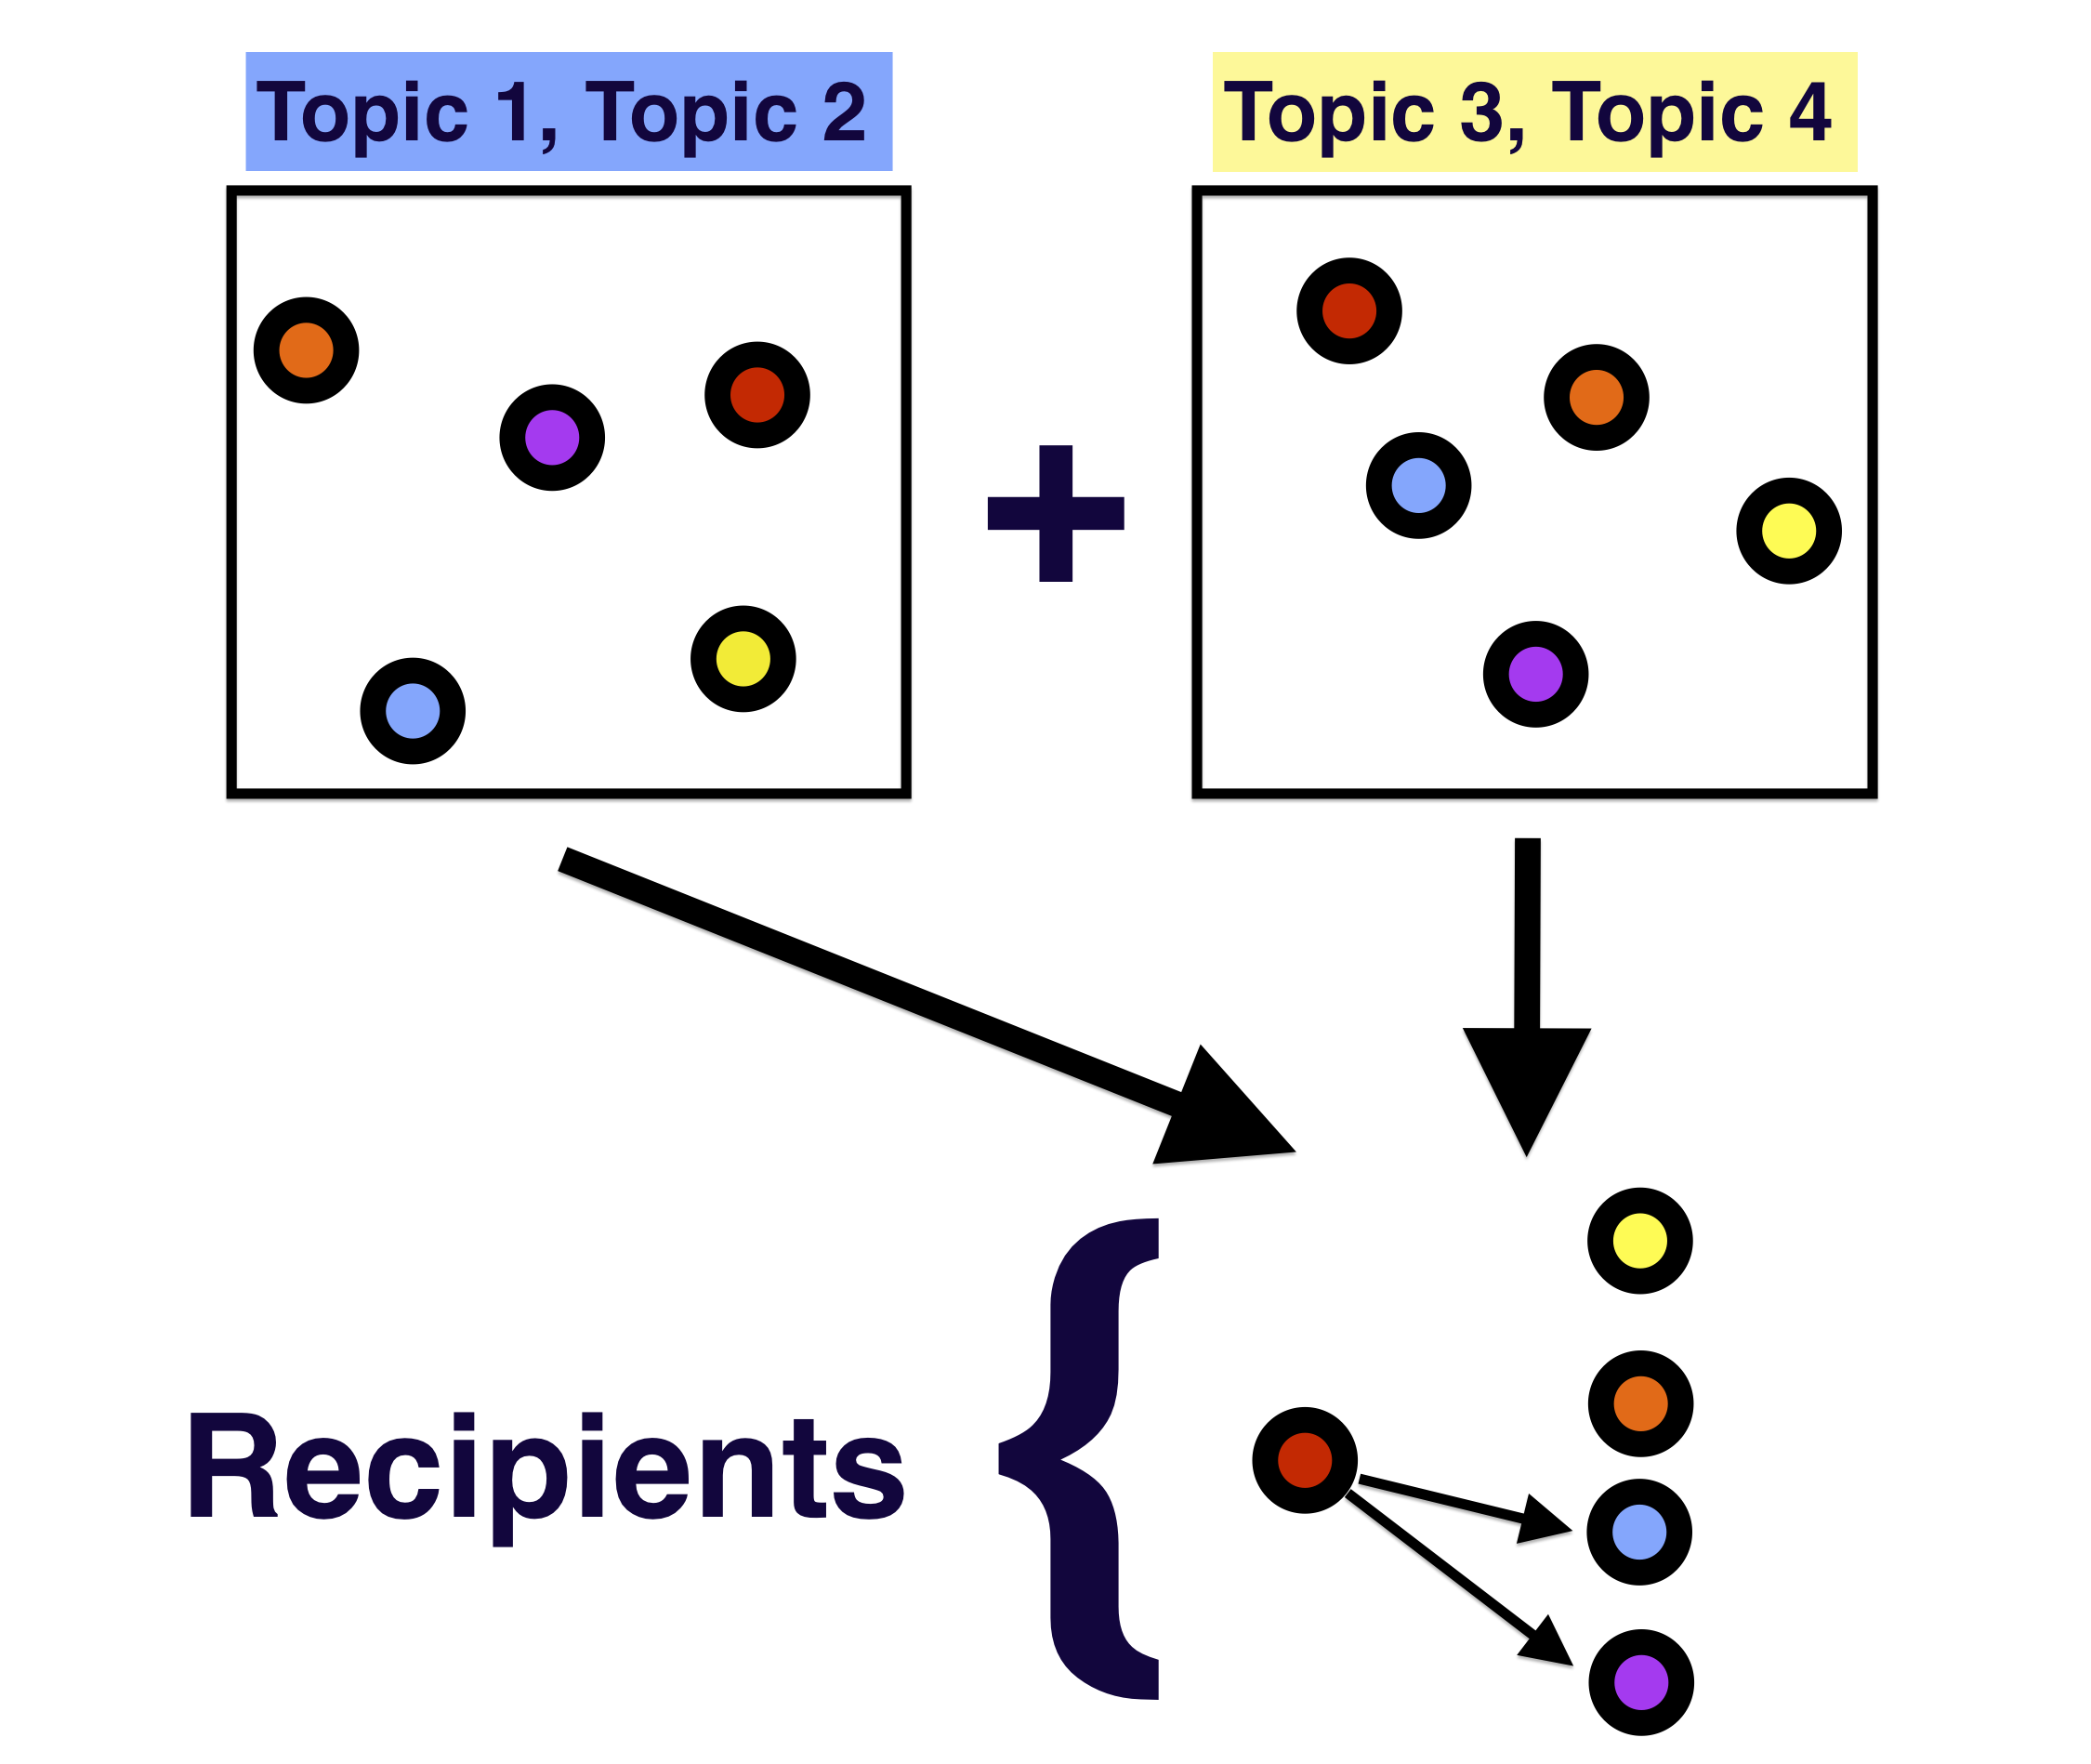
\includegraphics[width=0.92\textwidth]{images/Gen_Proc_3.png}
	\end{changemargin} 
\end{frame}

\begin{frame}\frametitle{Specification and Methods}
	\LARGE
	\begin{itemize}
		\item Bayesian inference via MCMC.
		\vspace*{.4in}
		\item Separate model for each county.
		\vspace*{.4in}
		\item Include gender mixing covariates.
		\vspace*{.4in}
		\item 40 topics, 4 interaction patterns.
		% \vspace*{.3in}
% 		\item Human code topics used in analysis.
	\end{itemize}
\end{frame}

\begin{frame}\frametitle{Example Model Output}
	
	\centering
	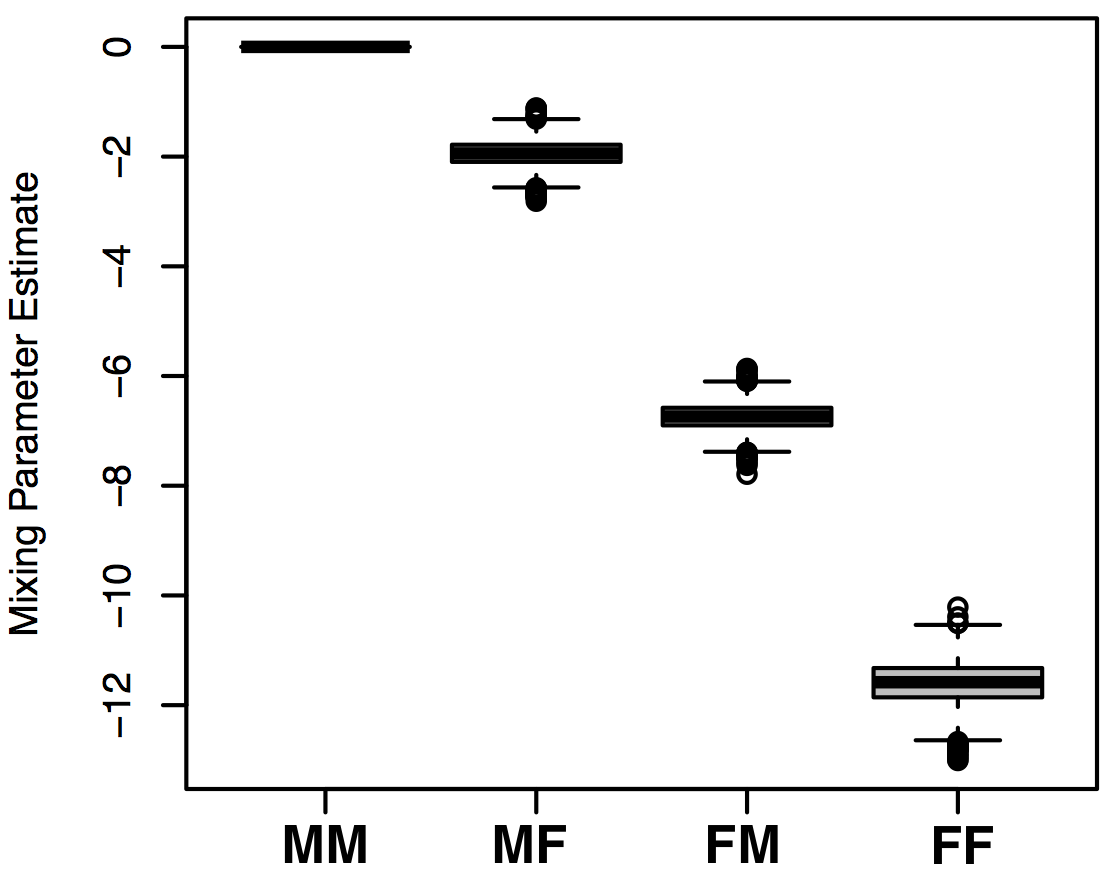
\includegraphics[width = .56\textwidth]{./images/Dare_3_MP.png}\\
	\begin{tabular}{l l}
	\toprule
	Coding & Topic top words\\
	\midrule
	\male{\textbf{Sandy}} & will, track, winds, system, forecast\\ 
	\male{\textbf{Sandy}} & storm, sandy, high, coastal, tides, night\\ 
	\male{\textbf{Harbor}} & status, update, boat, today, weather\\ 
	\male{\textbf{Planning}} & board, meeting, planning, seafood, hearing\\ 
	\male{\textbf{Storm}} & box, planning, director,  permit, building \\ 
	\bottomrule

	\end{tabular}
	
\end{frame}


\begin{frame}\frametitle{Female-Centric Topics of Communication}
	
	
\begin{changemargin}{-1cm}{ -1cm}	
	\centering
		\begin{tabular}{ll}
			\toprule
	Coding & FF $>$ FM $>$ MF $>$ MM\\
	\midrule

	\female{\textbf{Finance}} & order, time, good, april, attached, requests \\ 
	\female{\textbf{Finance}} & budget, phone, finance, media, ext, department
	\\ 
	\textbf{Health} & meeting, going, fyi, tricaster, health, project
	 \\ 
	\female{\textbf{Finance}} & meeting, box, fax, finance, attached, resolution
	\\ 
	\female{\textbf{Finance}} & equity, fax, debt, refunding, time, finance, call
	 \\ 
	\female{\textbf{Finance}} & debt, box, fax, finance, policies, contract, audit
	\\ 
	\female{\textbf{Finance}} & learn, leader, director, washington, dream
	\\ 
	\female{\textbf{Finance}} & fax, ext, phone, finance, director, street
	\\ 
	\textbf{Health} & public, health, email, contact, disclosure

	\\ 
	\female{\textbf{Finance}} & good, time, increase, call, pay, office, today
	
	\\ 
	\female{\textbf{Budget}} & manager, street, main, fax, office, east, budget
	
	\\ 
	\female{\textbf{Budget}} & fund, budget, balance, year, funds, pay, original
	
	\\

			\bottomrule
		\end{tabular}
		\end{changemargin}
\end{frame}






\begin{frame}\frametitle{Summary}
	\LARGE
	\begin{itemize}
		\item Micro-level behavioral data.
		\vspace*{.3in}
		\item Are women more active in female dominated domains?
		\vspace*{.3in}
		\item Different operationalizations of domain.
		\vspace*{.3in}
		\item Our results suggest this might be the case.
	\end{itemize}
\end{frame}



\begin{frame}\frametitle{Generative Process Pseudocode: Global Variables}
	\begin{changemargin}{-1cm}{ -1cm}
    \centering
	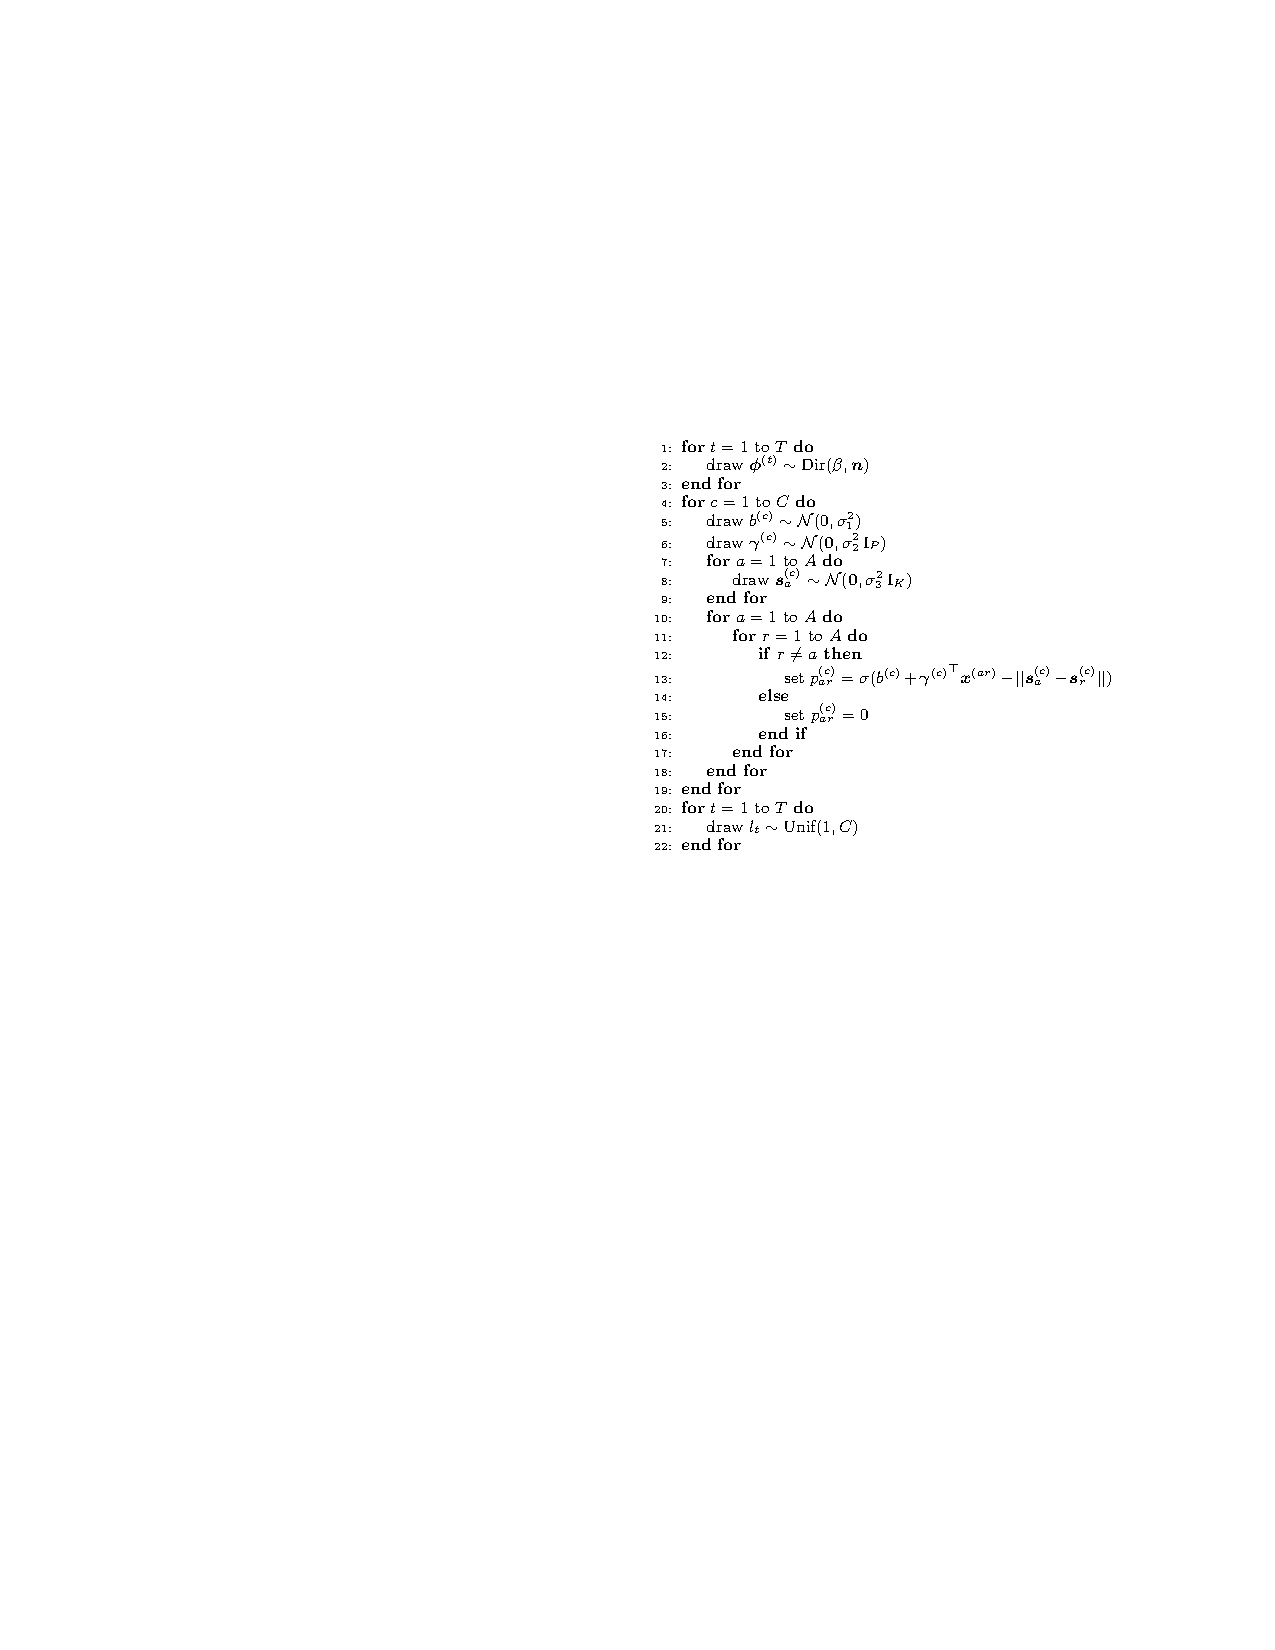
\includegraphics[width=.88\textwidth]{images/Pseudocode1.pdf}
	\end{changemargin} 
\end{frame}

\begin{frame}\frametitle{Generative Process Pseudocode: Local Variables}
	\begin{changemargin}{-1cm}{ -1cm}
    \centering
	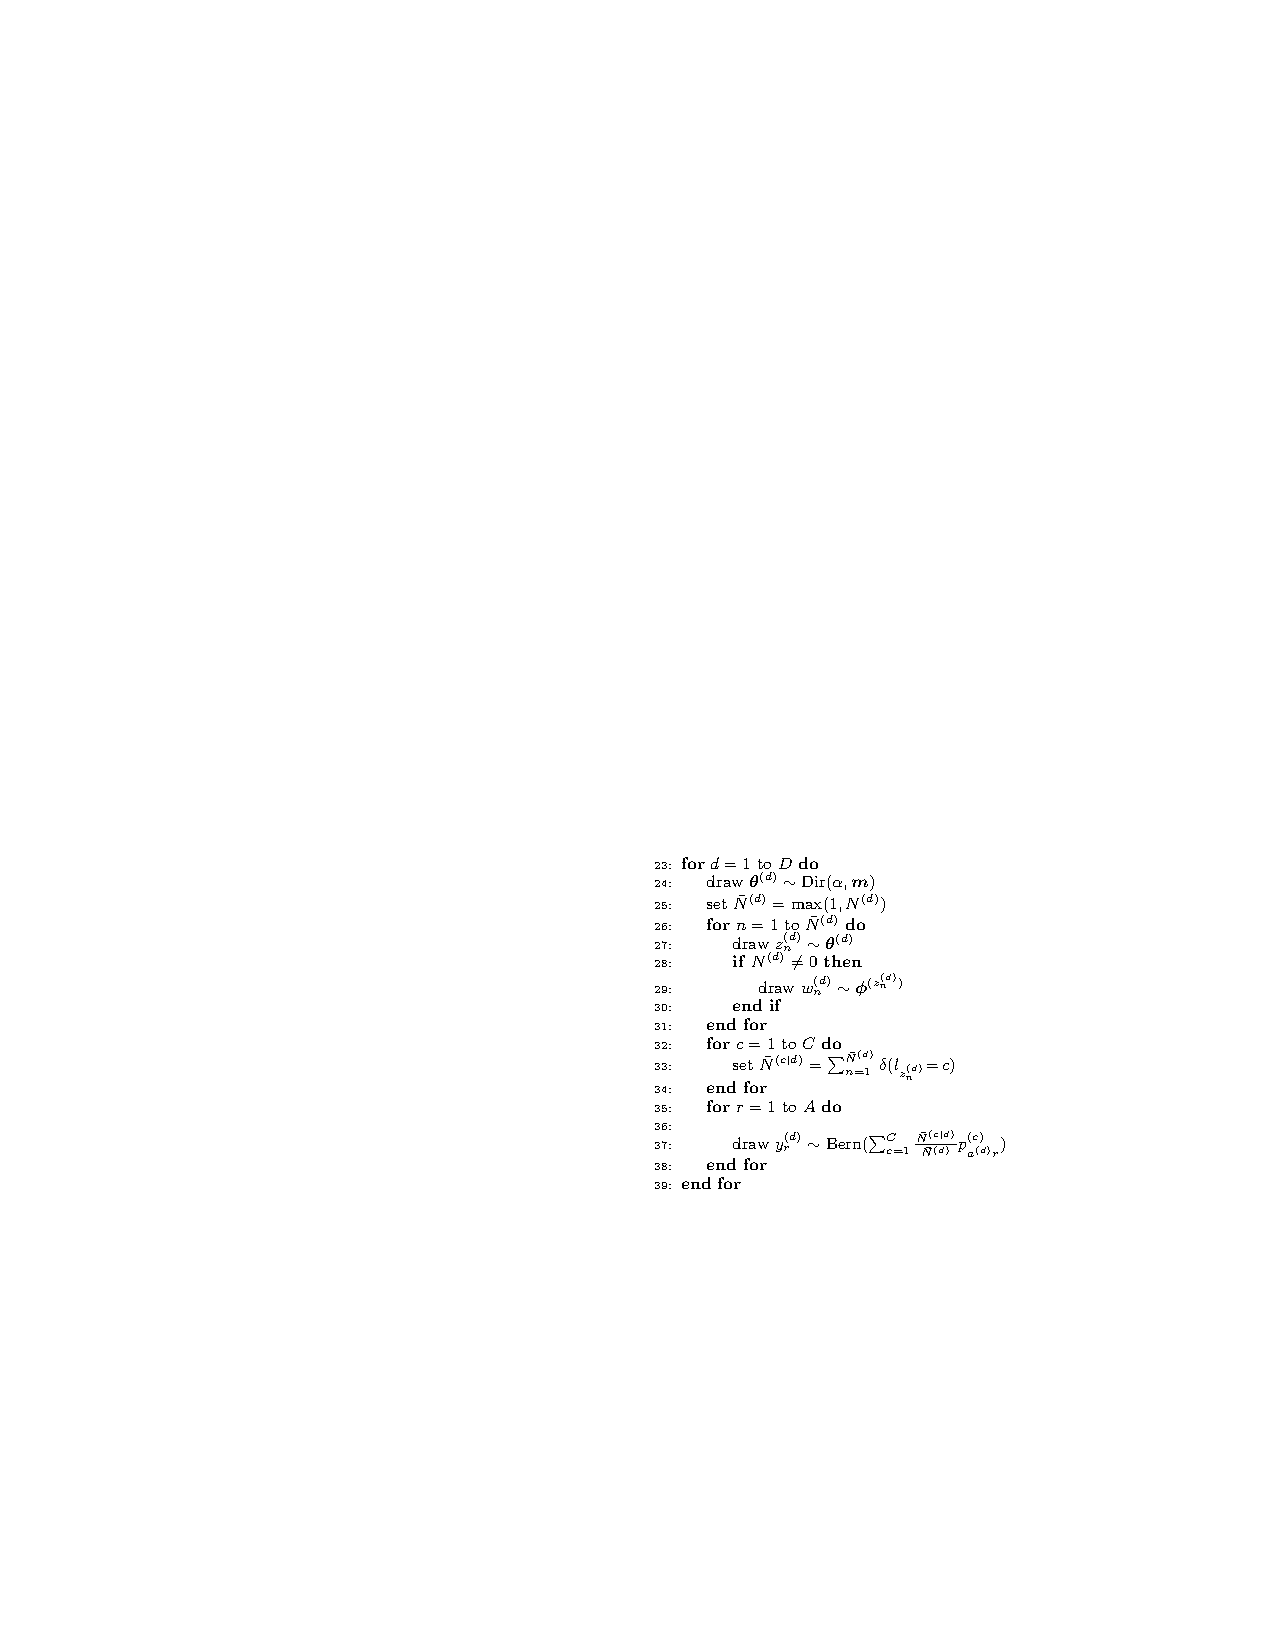
\includegraphics[width=.88\textwidth]{images/Pseudocode2.pdf}
	\end{changemargin} 
\end{frame}

\begin{frame}\frametitle{Inference Pseudocode}
	\begin{changemargin}{-1cm}{ -1cm}
    \centering
	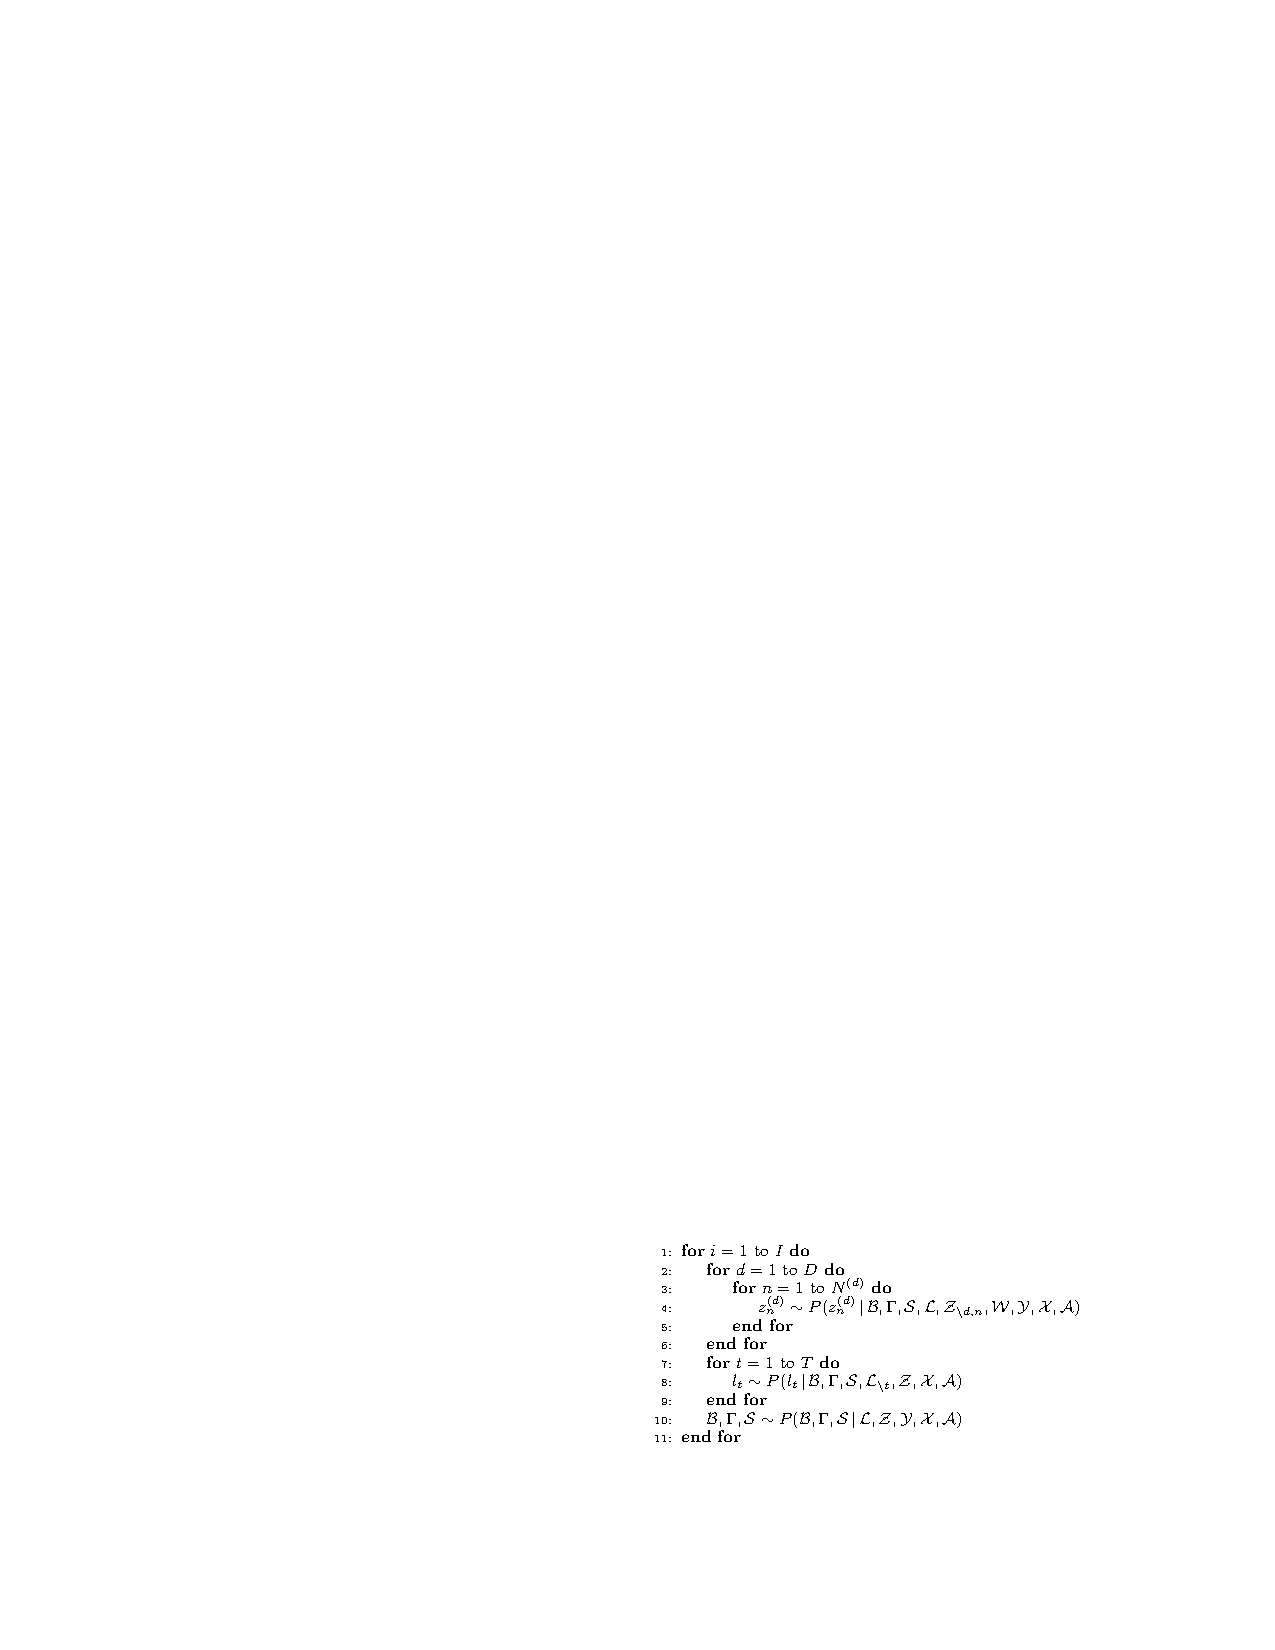
\includegraphics[width=.88\textwidth]{images/Pseudocode3.pdf}
	\end{changemargin} 
\end{frame}


\begin{frame}\frametitle{Human Coding Topics Used in Analysis}
	\LARGE
	\begin{itemize}
		\item Validate interpretation of top words
		\vspace*{.4in}
		\item Top ten emails.
		\vspace*{.2in}
		\begin{itemize}
			\LARGE
			\item Rank: $\frac{(\text{tokens assigned to topic})^2}{\text{tokens in email}}$
		\end{itemize}
		\vspace*{.2in}
		\item Label: common thread among emails.
		% \vspace*{.3in}
% 		\item Human code topics used in analysis.
	\end{itemize}
\end{frame}


\begin{frame}\frametitle{Male-Centric Dyads}
	\centering
	\Large
	\begin{tabular}{l}
	  \toprule
	  MM $>$ FM $>$ MF $>$ FF \\
	  \midrule
	  \male{Planning} \& \male{Information Technology} \\
	  \male{Solid Waste and Recycling} \& Health \\
	  \male{Sheriff} \& Health  \\
	  Tax Administrator \& \male{Planning}  \\
	  Tax Administrator \& Social Services  \\
	  \male{Inspections} \& Tax Administrator  \\
	  \male{Animal Control} \& \female{Finance}   \\
	  \male{Environment} \& Health  \\
	  \male{Environment} \& \male{Solid Waste and Recycling}  \\
	   \bottomrule
	\end{tabular}
\end{frame}



\begin{frame}\frametitle{Male-Centric Topics of Communication}
	
	
\begin{changemargin}{-.9cm}{ -1cm}	
	\centering
		\begin{tabular}{ll}
			\toprule
			Coding & MM $>$ FM $>$ MF $>$ FF\\
			  % & \\
			\midrule

	\male{\textbf{Manager}} & office, email, time, staff, meeting, work, good\\ 

	\male{\textbf{IT}} & electronic, mail, intended, email, message\\ 

	\textbf{Health} & health, department, project, email, code, garden\\ 


	\textbf{Comments} & jail, mobile, inmates, ago, money, jails\\ 

	\male{\textbf{Planning}} & east, planning, street, court, administrator\\ 


	\male{\textbf{Public Works}} & public, nashville, suite, washington\\ 


	\male{\textbf{Public Works}} & email, energy, carolina, north, address\\ 


	\male{\textbf{Planning}} & description, director, street, church, suite\\ 


	\male{\textbf{Planning}} & description, fax, phone, director, street, church\\ 


	\male{\textbf{Zoning}} & board, meeting, planning, amendment\\ 


	\male{\textbf{Emergency}} & operations, emergency, director, lines, street\\ 


	\textbf{Development} & description, director, development, projects\\ 

			\bottomrule
		\end{tabular}
		\end{changemargin}
\end{frame}




\end{document}
